
%---------------------- % % % Personnalisation des couleurs % % % ----------- BLEU --------
\definecolor{couleurFonce}{RGB}{0,92,133} % Couleur du Code APOGEE
\definecolor{couleurClaire}{RGB}{100,151,186} % Couleur du fond de la bande
\definecolor{couleurTexte}{RGB}{255,255,255} % Couleur du texte de la bande
%------------------------------------------------------------------------------------------



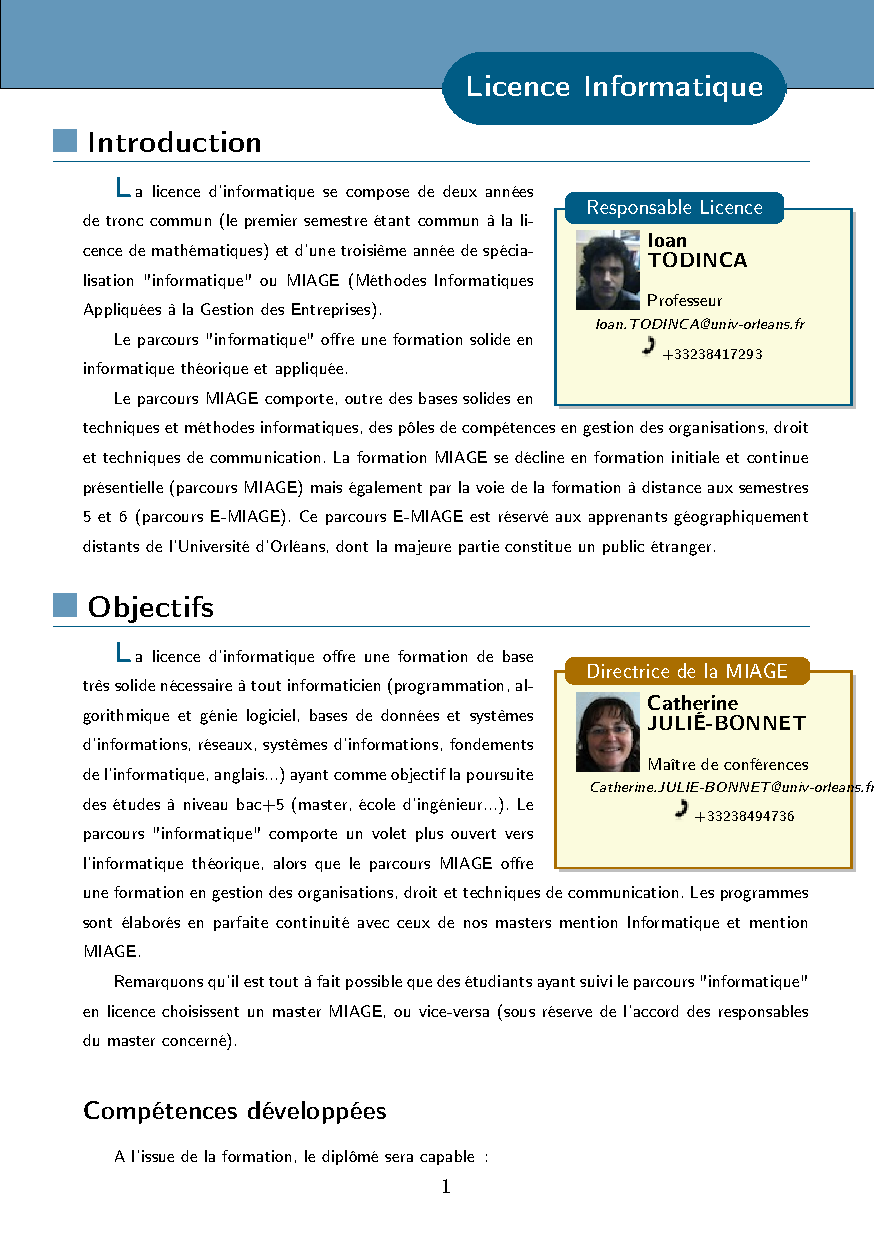
\includepdf[fitpaper,pages=-]{Preambule_Info_MasterMIAGE_SIMSA_S3S4.pdf}

%==========================================================================================
% Semestre 5 : INFO
%==========================================================================================

\module[codeApogee={UE 51}, 
titre={Mise à niveau informatique - PRL}, 
CODEUE={1}, 
COURS={}, 
TD={}, 
TP={12}, 
CTD={20}, 
TOTAL={32}, 
SEMESTRE={Semestre 5}, 
COEFF={0}, 
ECTS={0}, 
MethodeEval={Contrôle continue et terminal}, 
ModalitesCCSemestreUn={CC et CT}, 
ModalitesCCSemestreDeux={CT}, 
%CalculNFSessionUne={$\frac{(CC+2*CT)}{3}$}, 
%CalculNFSessionDeux={CT}, 
NoteEliminatoire={}, 
nomPremierResp={Catherine JULIÉ-BONNET}, 
emailPremierResp={Catherine.JULIE-BONNET@univ-orleans.fr}, 
nomSecondResp={}, 
emailSecondResp={}, 
langue={Français}, 
nbPrerequis={1}, 
descriptionCourte={true}, 
descriptionLongue={true}, 
objectifs={true}, 
ressources={true}, 
bibliographie={false}] 
{
Unité qui s\'intègre dans le PRL (Plan Réussite en Licence).\\
Obligatoire pour certains étudiants.
} 
{
Rappels sur l\'algorithmique et la programmation, les systèmes d\'exploitation, les outils de 
développement. 
} 
{Niveau bac + 2 en informatique ou équivalent.} 
{\begin{itemize}
 \ObjItem Remise à niveau essentiellement destinée aux étudiants intégrant la Licence au semestre 
5, afin de leur assurer les bases nécessaires pour suivre de manière satisfaisante les 
enseignements de troisième année.
\end{itemize} 
} 
{Ressources} 
{Biblio} 
 
\vfill

%==========================================================================================
\module[codeApogee={UE 52}, 
titre={Programmation avancée et structures dynamiques}, 
CODEUE={1}, 
COURS={18}, 
TD={30}, 
TP={}, 
CTD={}, 
TOTAL={48}, 
SEMESTRE={Semestre 5}, 
COEFF={5}, 
ECTS={5}, 
MethodeEval={Contrôle continue et terminal}, 
ModalitesCCSemestreUn={CC et CT}, 
ModalitesCCSemestreDeux={CT}, 
%CalculNFSessionUne={$\frac{(CC+2*CT)}{3}$}, 
%CalculNFSessionDeux={CT}, 
NoteEliminatoire={}, 
nomPremierResp={Jean-Jacques LACRAMPE}, 
emailPremierResp={Jean-Jacques.LACRAMPE@univ-orleans.fr}, 
nomSecondResp={}, 
emailSecondResp={}, 
langue={Français}, 
nbPrerequis={1}, 
descriptionCourte={true}, 
descriptionLongue={true}, 
objectifs={true}, 
ressources={true}, 
bibliographie={false}] 
{
Unité obligatoire. 
} 
{
Introduction au langage ADA. Types non contraints et pointeurs. Unités de compilation, modularité, généricité.
Tâches, rendez-vous, type protégés, répartition. Types étiquetés, programmation orientée objet, programmation par classe, héritage, héritage multiple.
Interfaçage : autres langages, interface graphique, serveur web,... 
} 
{Maîtrise de l\'algorithmique de base (y compris les techniques d\'assertion et d\'invariant) et des structures statiques.
Connaissance des principes de gestion mémoire, de la notion d\'état, de l\'affectation.
Expérience des entrées sorties (non-)bufferisées. } 
{\begin{itemize}
 \ObjItem Acquérir et combiner plusieurs méthodes de programmation au sein d\'un même langage.
 \ObjItem Intégrer la notion d\'abstraction des données et des traitements.
 \ObjItem Comprendre l\'intérêt du typage fort et de l\'induction de types.
 \ObjItem Arbitrer entre des solutions statiques et dynamiques. 
\end{itemize} 
} 
{Ressources} 
{Biblio} 
 
\vfill

%==========================================================================================
\module[codeApogee={UE 53}, 
titre={Réseaux}, 
CODEUE={1}, 
COURS={18}, 
TD={12}, 
TP={12}, 
CTD={}, 
TOTAL={42}, 
SEMESTRE={Semestre 5}, 
COEFF={4}, 
ECTS={4}, 
MethodeEval={Contrôle continue et terminal}, 
ModalitesCCSemestreUn={CC et CT}, 
ModalitesCCSemestreDeux={CT}, 
%CalculNFSessionUne={$\frac{(CC+2*CT)}{3}$}, 
%CalculNFSessionDeux={CT}, 
NoteEliminatoire={}, 
nomPremierResp={Abdelali ED-DBALI}, 
emailPremierResp={Abdelali.ED-DBALI@univ-orleans.fr}, 
nomSecondResp={}, 
emailSecondResp={}, 
langue={Français}, 
nbPrerequis={1}, 
descriptionCourte={true}, 
descriptionLongue={true}, 
objectifs={true}, 
ressources={true}, 
bibliographie={false}] 
{
Unité obligatoire. 
} 
{
Architecture des réseaux\,: structure en couches, protocoles, services. Réseaux locaux sous UDP-TCP/IP, Ethernet. Protocoles de routage\,: RIP, OSPF, BGP. Principaux protocoles Internet\,: DNS (annuaire de noms de domaines). SMTP (mail), FTP (transfert de fichiers), HTTP (web),... 
} 
{Algorithmique (modules de L1 et L2).} 
{\begin{itemize}
 \ObjItem Comprendre les principes et pratique des réseaux locaux informatiques.
 \ObjItem Être capable d\'installer et configurer un réseaux TCP/IP.
 \ObjItem Savoir configurer statiquement et dynamiquement un routeur.
\end{itemize} 
} 
{Ressources} 
{Biblio} 
 
\vfill

%==========================================================================================
\module[codeApogee={UE 54}, 
titre={Analyse des algorithmes}, 
CODEUE={1}, 
COURS={14}, 
TD={24}, 
TP={}, 
CTD={}, 
TOTAL={38}, 
SEMESTRE={Semestre 5}, 
COEFF={5}, 
ECTS={5}, 
MethodeEval={Contrôle continue et terminal}, 
ModalitesCCSemestreUn={CC et CT}, 
ModalitesCCSemestreDeux={CT}, 
%CalculNFSessionUne={$\frac{(CC+2*CT)}{3}$}, 
%CalculNFSessionDeux={CT}, 
NoteEliminatoire={}, 
nomPremierResp={Ioan TODINCA}, 
emailPremierResp={Ioan.TODINCA@univ-orleans.fr}, 
nomSecondResp={}, 
emailSecondResp={}, 
langue={Français}, 
nbPrerequis={1}, 
descriptionCourte={true}, 
descriptionLongue={true}, 
objectifs={true}, 
ressources={true}, 
bibliographie={false}] 
{
Unité obligatoire. 
} 
{
Complexité d\'un algorithme. Diviser pour régner. Algorithmes gloutons. Programmation dynamique. Algorithmes de tri ; arbres binaires de recherche. 
} 
{algorithmique et programmation élémentaire} 
{\begin{itemize}
 \ObjItem Maîtriser les techniques algorithmiques de base (diviser pour régner, algorithmes gloutons...).
 \ObjItem Savoir analyser la complexité d\'un algorithme. 
\end{itemize} 
} 
{Ressources} 
{Biblio} 
 
\vfill

%==========================================================================================
\module[codeApogee={UE 55}, 
titre={Programmation linéaire}, 
CODEUE={1}, 
COURS={14}, 
TD={20}, 
TP={4}, 
CTD={}, 
TOTAL={38}, 
SEMESTRE={Semestre 5}, 
COEFF={4}, 
ECTS={4}, 
MethodeEval={Contrôle continue et terminal}, 
ModalitesCCSemestreUn={CC et CT}, 
ModalitesCCSemestreDeux={CT}, 
%CalculNFSessionUne={$\frac{(CC+2*CT)}{3}$}, 
%CalculNFSessionDeux={CT}, 
NoteEliminatoire={}, 
nomPremierResp={Ioan TODINCA}, 
emailPremierResp={Ioan.TODINCA@univ-orleans.fr}, 
nomSecondResp={}, 
emailSecondResp={}, 
langue={Français}, 
nbPrerequis={1}, 
descriptionCourte={true}, 
descriptionLongue={true}, 
objectifs={true}, 
ressources={true}, 
bibliographie={false}] 
{
Unité obligatoire. 
} 
{
modélisation de problèmes linéaires\,; résolution graphique\,; algorithme du simplexe\,; méthode du simplexe ; dualité ; théorème de dualité ; théorème des écarts complémentaires\,; interprétation économique du dual\,; études de cas\,; programmation 
linéaire en nombres entiers. 
} 
{Algèbre et Algorithmique de L1 et L2.} 
{\begin{itemize}
 \ObjItem Être capable de à modéliser et résoudre des problèmes d\'optimisation linéaire. 
\end{itemize} 
} 
{Ressources} 
{Biblio} 
 
\vfill

%==========================================================================================
\module[codeApogee={UE 56 }, 
titre={Logique}, 
CODEUE={1}, 
COURS={12}, 
TD={18}, 
TP={}, 
CTD={}, 
TOTAL={30}, 
SEMESTRE={Semestre 5}, 
COEFF={3}, 
ECTS={3}, 
MethodeEval={Contrôle continue et terminal}, 
ModalitesCCSemestreUn={CC et CT}, 
ModalitesCCSemestreDeux={CT}, 
%CalculNFSessionUne={$\frac{(CC+2*CT)}{3}$}, 
%CalculNFSessionDeux={CT}, 
NoteEliminatoire={}, 
nomPremierResp={Thi Bich Hanh DIEP DAO}, 
emailPremierResp={Thi-Bich-Hanh.DAO@univ-orleans.fr}, 
nomSecondResp={}, 
emailSecondResp={}, 
langue={Français}, 
nbPrerequis={0}, 
descriptionCourte={true}, 
descriptionLongue={true}, 
objectifs={true}, 
ressources={true}, 
bibliographie={false}] 
{
Unité obligatoire. 
} 
{
Calcul des propositions, calcul des prédicats, sémantique, modèle. Théorie de la démonstration, déduction naturelle, unification, méthode de résolution. 
} 
{} 
{\begin{itemize}
 \ObjItem Comprendre et maîtriser la logique mathématique pour l\'informatique.
\end{itemize} 
} 
{Ressources} 
{Biblio} 
 
\vfill

%==========================================================================================
\module[codeApogee={UE 57 }, 
titre={Systèmes d\'information}, 
CODEUE={1}, 
COURS={12}, 
TD={12}, 
TP={6}, 
CTD={}, 
TOTAL={30}, 
SEMESTRE={Semestre 5}, 
COEFF={3}, 
ECTS={3}, 
MethodeEval={Contrôle continue et terminal}, 
ModalitesCCSemestreUn={CC et CT}, 
ModalitesCCSemestreDeux={CT}, 
%CalculNFSessionUne={$\frac{(CC+2*CT)}{3}$}, 
%CalculNFSessionDeux={CT}, 
NoteEliminatoire={}, 
nomPremierResp={Raymond RAKOTOZAFY}, 
emailPremierResp={Raymond.RAKOTOZAFY@univ-orleans.fr}, 
nomSecondResp={}, 
emailSecondResp={}, 
langue={Français}, 
nbPrerequis={0}, 
descriptionCourte={true}, 
descriptionLongue={true}, 
objectifs={true}, 
ressources={true}, 
bibliographie={false}] 
{
Unité obligatoire. 
} 
{
Étude des concepts fondamentaux utilisés par un système d\'information et études de cas.
} 
{} 
{\begin{itemize}
 \ObjItem Acquisition des concepts de base des systèmes d\'informations. 
 \ObjItem Capacité à mener une analyse des besoins d\'une société en termes de systèmes d\'information. 
 \ObjItem Utilisation concrète d\'une méthode et application à des études de cas.
\end{itemize} 
} 
{Ressources} 
{Biblio} 
 
\vfill

%==========================================================================================
\module[codeApogee={UE 58 }, 
titre={Anglais 5}, 
CODEUE={1}, 
COURS={}, 
TD={25}, 
TP={}, 
CTD={}, 
TOTAL={25}, 
SEMESTRE={Semestre 5}, 
COEFF={3}, 
ECTS={3}, 
MethodeEval={Contrôle continue et terminal}, 
ModalitesCCSemestreUn={CC et CT}, 
ModalitesCCSemestreDeux={CT}, 
%CalculNFSessionUne={$\frac{(CC+2*CT)}{3}$}, 
%CalculNFSessionDeux={CT}, 
NoteEliminatoire={}, 
nomPremierResp={Hervé PERREAU}, 
emailPremierResp={Herve.PERREAU@univ-orleans.fr}, 
nomSecondResp={}, 
emailSecondResp={}, 
langue={Français}, 
nbPrerequis={1}, 
descriptionCourte={true}, 
descriptionLongue={true}, 
objectifs={true}, 
ressources={true}, 
bibliographie={false}] 
{
Unité obligatoire. 
} 
{
Travail de compréhension et d’expression à partir de documents authentiques longs et/ou complexes portant sur des innovations technologiques, des découvertes et avancées scientifiques.
} 
{Avoir suivi les unités Anglais 3 et 4 ou un volume d\'heures de formation équivalente.} 
{\begin{itemize} 
 \ObjItem Comprendre l’information exprimée dans des messages complexes sur le domaine des Sciences et Technologies et s’exprimer sur ce même domaine à l’écrit dans un registre de langue approprié. 
\end{itemize} 
} 
{Ressources} 
{Biblio} 
 
\vfill

%==========================================================================================
\module[codeApogee={UE 59 }, 
titre={Unité Libre}, 
CODEUE={1}, 
COURS={}, 
TD={24}, 
TP={}, 
CTD={}, 
TOTAL={24}, 
SEMESTRE={Semestre 5}, 
COEFF={3}, 
ECTS={3}, 
MethodeEval={Contrôle continue et terminal}, 
ModalitesCCSemestreUn={CC et CT}, 
ModalitesCCSemestreDeux={CT}, 
%CalculNFSessionUne={$\frac{(CC+2*CT)}{3}$}, 
%CalculNFSessionDeux={CT}, 
NoteEliminatoire={}, 
nomPremierResp={Scolarité des Sciences}, 
emailPremierResp={}, 
nomSecondResp={}, 
emailSecondResp={}, 
langue={Français}, 
nbPrerequis={0}, 
descriptionCourte={true}, 
descriptionLongue={true}, 
objectifs={true}, 
ressources={true}, 
bibliographie={false}] 
{
Unité obligatoire. 
} 
{
L\'unité Libre est à choisir, en début du semestre, parmi la centaine d\'enseignements dédiés à cet usage et offerts par toutes
les composantes de l\'université (Sciences, Droit-Economie-Gestion, Sport).\\
Voici quelques exemples d\'unités Libres\,:
\begin{itemize}
  \item Sport.
  \item Droit de l\'informatique.
  \item Problèmes économiques contemporains.
  \item Histoire du cinéma, histoire des arts.
  \item Enseigner : posture et identité professionnelles.
  \item Lecture critique du réchauffement climatique.
  \item Maîtriser son expression ; les enjeux de la communication orale : le corps, l\'espace, la voix.
\end{itemize} 
} 
{}
{\begin{itemize}
 \ObjItem Comprendre comment ce qu\'on apprend dans le cadre d\'un diplôme déjà très spécialisé s\'insère dans le large champ des connaissances
 et des savoirs auxquels on sera confronté dans son expérience professionnelle ou personnelle.
\end{itemize} 
} 
{La page du site de l\'université dédiée aux unités Libres: http://www.univ-orleans.fr/scolarite/inscriptions/?page=2} 
{Biblio} 
 
\vfill

%==========================================================================================
% Semestre 6 : INFO
%==========================================================================================

\module[codeApogee={UE 61}, 
titre={Renforcement POO Java}, 
CODEUE={1}, 
COURS={}, 
TD={}, 
TP={12}, 
CTD={}, 
TOTAL={12}, 
SEMESTRE={Semestre 6}, 
COEFF={0}, 
ECTS={0}, 
MethodeEval={Contrôle continue et terminal}, 
ModalitesCCSemestreUn={CC et CT}, 
ModalitesCCSemestreDeux={CT}, 
%CalculNFSessionUne={$\frac{(CC+2*CT)}{3}$}, 
%CalculNFSessionDeux={CT}, 
NoteEliminatoire={}, 
nomPremierResp={Frédéric MOAL}, 
emailPremierResp={Frederic.MOAL@univ-orleans.fr}, 
nomSecondResp={}, 
emailSecondResp={}, 
langue={Français}, 
nbPrerequis={0}, 
descriptionCourte={true}, 
descriptionLongue={true}, 
objectifs={true}, 
ressources={true}, 
bibliographie={false}] 
{
Unité qui s\'intègre dans le PRL (Plan Réussite en Licence).\\
Obligatoire pour certains étudiants.
} 
{
Programmation orientée objet. Gestion de la mémoire. 
} 
{} 
{\begin{itemize}
  \ObjItem Assainir les lacunes encore présentes en programmation.
\end{itemize}
} 
{Ressources} 
{Biblio} 
 
\vfill

%==========================================================================================
\module[codeApogee={UE 62}, 
titre={Génie Logiciel}, 
CODEUE={1}, 
COURS={12}, 
TD={20}, 
TP={8}, 
CTD={}, 
TOTAL={40}, 
SEMESTRE={Semestre 6}, 
COEFF={5}, 
ECTS={5}, 
MethodeEval={Contrôle continue et terminal}, 
ModalitesCCSemestreUn={CC et CT}, 
ModalitesCCSemestreDeux={CT}, 
%CalculNFSessionUne={$\frac{(CC+2*CT)}{3}$}, 
%CalculNFSessionDeux={CT}, 
NoteEliminatoire={}, 
nomPremierResp={Laure KAHLEM}, 
emailPremierResp={Laure.KAHLEM@univ-orleans.fr}, 
nomSecondResp={}, 
emailSecondResp={}, 
langue={Français}, 
nbPrerequis={1}, 
descriptionCourte={true}, 
descriptionLongue={true}, 
objectifs={true}, 
ressources={true}, 
bibliographie={false}] 
{
Unité obligatoire. 
} 
{
Généralités, cycle de vie d\'un logiciel, méthodes d\'analyse et de conception, méthodes objet, langage UML, méthodes de tests. 
} 
{Notions de modélisation et de système d\'information} 
{\begin{itemize}
  \ObjItem Acquérir une connaissance des outils et des techniques de spécification tels que les réseaux de Petri. Maîtriser un langage dédié au génie logiciel, UML.
\end{itemize} 
} 
{Ressources} 
{Biblio} 
 
\vfill

%==========================================================================================
\module[codeApogee={UE 63}, 
titre={Bases de données}, 
CODEUE={1}, 
COURS={12}, 
TD={20}, 
TP={8}, 
CTD={}, 
TOTAL={40}, 
SEMESTRE={Semestre 6}, 
COEFF={4}, 
ECTS={4}, 
MethodeEval={Contrôle continue et terminal}, 
ModalitesCCSemestreUn={CC et CT}, 
ModalitesCCSemestreDeux={CT}, 
%CalculNFSessionUne={$\frac{(CC+2*CT)}{3}$}, 
%CalculNFSessionDeux={CT}, 
NoteEliminatoire={}, 
nomPremierResp={Khalil DJELLOUL}, 
emailPremierResp={Khalil.DJELLOUL@univ-orleans.fr}, 
nomSecondResp={}, 
emailSecondResp={}, 
langue={Français}, 
nbPrerequis={1}, 
descriptionCourte={true}, 
descriptionLongue={true}, 
objectifs={true}, 
ressources={true}, 
bibliographie={false}] 
{
Unité obligatoire. 
} 
{
Algèbre relationnelle. SQL : Langage d\'Interrogation des Données. Dépendances fonctionnelles et Formes normales. SQL : Langage de Définition des Données. Mise en \oe uvre des contraintes d\'intégrité avec Oracle 
} 
{UE : Bases des données et internet (L2).} 
{\begin{itemize} 
 \ObjItem Créer des bases de données relationnelles d\'une bonne forme normale. 
 \ObjItem Mettre en \oe uvre des contraintes d\'intégrité au sein de bases de données relationnelles. 
 \ObjItem Interroger des bases de données relationnelles. 
\end{itemize} 
} 
{Ressources} 
{Biblio} 
 
\vfill

%==========================================================================================
\module[codeApogee={UE 64}, 
titre={Théorie des langages}, 
CODEUE={1}, 
COURS={14}, 
TD={26}, 
TP={}, 
CTD={}, 
TOTAL={40}, 
SEMESTRE={Semestre 6}, 
COEFF={4}, 
ECTS={4}, 
MethodeEval={Contrôle continue et terminal}, 
ModalitesCCSemestreUn={CC et CT}, 
ModalitesCCSemestreDeux={CT}, 
%CalculNFSessionUne={$\frac{(CC+2*CT)}{3}$}, 
%CalculNFSessionDeux={CT}, 
NoteEliminatoire={}, 
nomPremierResp={Wadoud BOUSDIRA}, 
emailPremierResp={Wadoud.BOUSDIRA@univ-orleans.fr}, 
nomSecondResp={}, 
emailSecondResp={}, 
langue={Français}, 
nbPrerequis={1}, 
descriptionCourte={true}, 
descriptionLongue={true}, 
objectifs={true}, 
ressources={true}, 
bibliographie={false}] 
{
Unité obligatoire. 
} 
{
généralités sur monoïde, langages et grammaires formels ; classification de Chomsky ; langages réguliers ; grammaires régulières ; automates finis ; déterminisation d\'automates finis ; expressions régulières ; résolution de systèmes d\'équations linéaires ; théorème de Kleene ; automate minimal ; minimisation d\'automates finis ; lemme d\'itération. 
} 
{notions de bases en algèbre et théorie des graphes} 
{\begin{itemize}
  \ObjItem notions de base sur les langages réguliers et automates finis, préparation à l\'enseignement de compilation.
\end{itemize} 
} 
{Ressources} 
{Biblio} 
 
\vfill

%==========================================================================================
\module[codeApogee={UE 65}, 
titre={Projet informatique 3}, 
CODEUE={1}, 
COURS={6}, 
TD={}, 
TP={}, 
CTD={}, 
TOTAL={6}, 
SEMESTRE={Semestre 6}, 
COEFF={6}, 
ECTS={6}, 
%MethodeEval={Contrôle continue et terminal}, 
ModalitesCCSemestreUn={Rapport et soutenance de projet}, 
ModalitesCCSemestreDeux={Pas de 2nde session}, 
%CalculNFSessionUne={$\frac{(CC+2*CT)}{3}$}, 
%CalculNFSessionDeux={CT}, 
NoteEliminatoire={}, 
nomPremierResp={Ioan TODINCA}, 
emailPremierResp={Ioan.TODINCA@univ-orleans.fr}, 
nomSecondResp={}, 
emailSecondResp={}, 
langue={Français}, 
nbPrerequis={0}, 
descriptionCourte={true}, 
descriptionLongue={true}, 
objectifs={true}, 
ressources={true}, 
bibliographie={false}] 
{
Unité obligatoire. 
} 
{
Projet de fin d\'études, faisant intervenir différentes connaissances et compétences acquises lors de l\'ensemble de la formation en licence.
} 
{Niveau de connaissance et de compétence de fin d\'année de licence (L3), en particulier dans les domaines de l\'analyse, de la modélisation et de la programmation.
Le langage de programmation souhaité pour le projet devra être connu ou maîtrisé dans un délai très court.
De plus il est obligatoire de s\'impliquer dans un groupe de travail et de posséder un minimum de qualités dans la communication.
} 
{\begin{itemize} 
 \ObjItem Au sein d\'un groupe, apprendre à organiser la réalisation complète d\'un projet, depuis l\'analyse jusqu\'aux tests de validation en utilisant des outils collaboratifs. 
 \ObjItem Percevoir les différentes compétences nécessaires au sein d\'un groupe de travail Se préparer au métier de chef de projet. 
\end{itemize} 
} 
{Ressources} 
{Biblio} 
 
\vfill

%==========================================================================================
\module[codeApogee={UE 66},
titre={Anglais 6},
CODEUE={1},
COURS={},
TD={25},
TP={},
CTD={},
TOTAL={25},
SEMESTRE={Semestre 6},
COEFF={3},
ECTS={3},
MethodeEval={Contrôle continue et terminal},
ModalitesCCSemestreUn={CC et CT},
ModalitesCCSemestreDeux={CT},
%CalculNFSessionUne={$\frac{(CC+2*CT)}{3}$},
%CalculNFSessionDeux={CT},
NoteEliminatoire={},
nomPremierResp={Hervé PERREAU},
emailPremierResp={Hervé.PERREAU@univ-orleans.fr},
nomSecondResp={},
emailSecondResp={},
langue={Français},
nbPrerequis={1},
descriptionCourte={true},
descriptionLongue={true},
objectifs={true},
ressources={true},
bibliographie={false}]
{
Unité obligatoire.
}
{
Travail de compréhension et d’expression à partir de documents authentiques longs et/ou complexes portant sur des innovations technologiques, des découvertes et avancées scientifiques.
} 
{Avoir suivi l\'unité "Anglais 5" ou un volume d\'heures de formation équivalente.} 
{\begin{itemize} 
 \ObjItem Comprendre l’information exprimée dans des messages complexes sur le domaine des Sciences et Technologies et s’exprimer sur ce même domaine à l’oral avec un degré suffisant de spontanéité et de fluidité (niveau européen\,: B2). 
\end{itemize} 
} 
{Ressources} 
{Biblio} 
 
\vfill

%==========================================================================================
\module[codeApogee={UE 69},
titre={Stage ou projet de fin d\'études},
CODEUE={1},
COURS={},
TD={},
TP={},
CTD={},
TOTAL={3 mois},
SEMESTRE={Semestre 6},
COEFF={8},
ECTS={8},
%MethodeEval={Contrôle continue et terminal},
ModalitesCCSemestreUn={Rapport et soutenance de stage ou de projet},
ModalitesCCSemestreDeux={Pas de 2nde session},
%CalculNFSessionUne={$\frac{(CC+2*CT)}{3}$},
%CalculNFSessionDeux={CT},
NoteEliminatoire={},
nomPremierResp={Khalil DJELLOUL},
emailPremierResp={Khalil.DJELLOUL@univ-orleans.fr},
nomSecondResp={Ioan TODINCA}, 
emailSecondResp={Ioan.TODINCA@univ-orleans.fr}, 
langue={Français}, 
nbPrerequis={1}, 
descriptionCourte={true}, 
descriptionLongue={true}, 
objectifs={true}, 
ressources={true}, 
bibliographie={false}] 
{
Unité obligatoire. 
} 
{
Stage d\'au moins trois mois consécutifs dans une entreprise ou projet de fin d\'étude, suivi par un enseignant et donnant lieu à la rédaction d\'un mémoire puis d\'une soutenance de stage en présence d\'un jury mixte d\'enseignants et de responsables de l\'entreprise. 
} 
{Compétences acquises au cours de la licence.} 
{\begin{itemize}
  \ObjItem Capacité à participer et mener à bien un projet au sein d\'une entreprise.
  \ObjItem Connaissance du monde professionnel.
\end{itemize} 
} 
{Ressources} 
{Biblio} 
 
\vfill
